\documentclass{article}

% Target journal: Molecular Phylogenetics and Evolution
%
% From author guidelines:
%
% Short communications of approximately 3000 words are also accepted. 
% These papers should contain no more than two figures, two tables, and thirty references. 
% A short abstract of fewer than 200 words is acceptable.


% Annotation/feedback commands
\newcommand*\rampal[1]{\textcolor{red}{\textbf{[RSE: #1]}}}
\newcommand*\richel[1]{\textcolor{orange}{\textbf{[RJCB: #1]}}}
\newcommand*\gio[1]{\textcolor{green}{\textbf{[GL: #1]}}}

% Bibliography
\usepackage{natbib}
\bibpunct{(}{)}{;}{a}{}{;}

\usepackage{amssymb}
\usepackage[english]{babel}

% Use 'It was found that something is something (Name 1234)' style
\setcitestyle{authoryear,open={},close={}}

% Affiliations
\usepackage{authblk}
\title{The error in Bayesian phylogenetic reconstruction when speciation co-occurs}

\author[1]{Giovanni Laudanno}
\author[1]{Rich\`el J.C. Bilderbeek}
\author[1]{Rampal S. Etienne}
\affil[1]{Groningen Institute for Evolutionary Life Sciences, University of Groningen, Groningen, The Netherlands}

% Use double spacing
\usepackage{setspace}
\doublespacing

\usepackage{pgf}
\usepackage{hyperref}
\usepackage{verbatim}
\usepackage{comment}
  
% Adds numbered lines
\usepackage{lineno}
\linenumbers

\hyphenation{
  BEAST
  Pa-ra-me-ter
  Drum-mond 
  Bayes-ian 
  Mr-Bayes 
  ap-proach-es 
  Rev-Bayes 
  cre-ate
  spe-ci-a-tion-com-ple-tion
  pro-trac-ted
 }

\begin{document}

\maketitle

%%%%%%%%%%%%%%%%%%%%%%%%%%%%%%%%%%%%%%%%%%%%%%%%%%%%%%%%%%%%%%%%%%%%%%%%%%%%%%%%
\begin{abstract}

  % From 'How to construct a Nature summary paragraph'

  % A short abstract of fewer than 200 words is acceptable.

  % One or two sentences providing a basic
  % introduction to the field,
  % comprehensible to a scientist in any discipline.
  

  % Two to three sentences of
  % more detailed background, comprehensible to
  % scientists in related disciplines.
  

  % One sentence clearly stating the general
  % problem being addressed by this particular
  % study.
  

  % One sentence summarising the main
  % result (with the words “here we show”
  % their equivalent).
  

  % Two or three sentences explaining what
  % the main result reveals in direct
  % comparison to what was thought to be the case
  % previously, or how the main result adds to
  % previous knowledge.

  % One or two sentences to put the results into a
  % more general context.


  % Two or three sentences to provide a
  % broader perspective, readily comprehensible
  % to a scientist in any discipline, may be included
  % in the first paragraph if the editor considers that the accessibility of the paper is significantly enhanced
  % by their inclusion. Under these circumstances, the length of the paragraph can be up to 300 words.
  % (The above example is 190 words without the final section, and 250 words with it).



\end{abstract}

{\bf Keywords:} computational biology, evolution, phylogenetics, Bayesian analysis, tree prior
%%%%%%%%%%%%%%%%%%%%%%%%%%%%%%%%%%%%%%%%%%%%%%%%%%%%%%%%%%%%%%%%%%%%%%%%%%%%%%%%
\richel{Have you already looked up for a target journal?} 
\gio{Honestly I have literally no idea how to select a good journal for this kind of article.}
\richel{
  May I suggest we aim for Molecular Phylogenetics and Evolution, the same journal as the raket paper?
} 

%%%%%%%%%%%%%%%%%%%%%%%%%%%%%%%%%%%%%%%%%%%%%%%%%%%%%%%%%%%%%%%%%%%%%%%%%%%%%%%%
\section{Introduction}
\begin{itemize}

\item There are many contemporary tools that provide the possibility 
to infer a phylogeny from genetic data (DNA, RNA, proteins). 
A popular Bayesian phylogenetic tool is called BEAST (\cite{beast}) 
and its cousin BEAST2 (\cite{beast2}).

\item BEAST is very flexible, providing the user with the option 
to set up all possible phylogenetic priors (e.g. site/clock/speciation model).

%Current limits in current tools.
\item However, currently available priors can be not suitable 
to analyze some specific datasets. 
With this work we aim to test whether or not 
the implementation of a new prior model 
is beneficial to study a specific kind of diversification process.

\item BEAST2 gives us the possibility to introduce new tree priors 
to infer phylogenies based on different assumptions 
on how the speciation process takes place.

\item One of such speciation processes is the multiple birth hypothesis,
a new model (described below) and thus currently absent in BEAST.

\item The Multiple birth hypothesis can be useful to explain a phenomenon 
that has always puzzled evolutionary biologists: 
what are the drivers of the diversification processes 
for those phylogenies that show an impressive amount of speciation events 
in relatively short times? 
The (constant-rate) birth-death (BD) model embodies the common assumption that 
only a single speciation event can occur at any given time.
The multiple-birth-death (MBD) model 
relaxes this assumption, allowing events in which 
large-scale environmental changes lead to a great number of species 
in relatively short time intervals. 
Such a hypothesis may be a better fit to describe the burst in systems 
like cichlid fish diversification in the 
African Great Lakes: Malawi, Tanganyika and Victoria 
(\cite{janzen2016}, \cite{janzen2017}).

\item However, it may be that current BD tree priors are good enough 
at detecting such events, with a (preferred) lower level of complexity. 
If this is the case one should always be more keen to adopt the simplest model.

\item Here we present our study with the aim of exploring 
when using a more complex MBD tree prior is warranted.

% Hypothesis: general
\item We hypothesize that the error made today, using BD tree priors,
increases with an increased number or stronger effect of multiple birth events.
This is straightforward: without multiple birth events or such event having
no effect, the MBD model falls back to a BD model. We expect larger
errors when we deviate more from the BD model's assumptions. 

\item Additionally, we hypothesize MBD having a stronger effect if the normal
speciation process is less pronounced. The more speciations are caused by the
BD process, there are relatively less multiple-birth events. 

\item We expect the effect of extinction rates to be neutral, as extinctions will
hit lineages created by both speciation processes equally. 

\item Summarized, we expect the error made be correlated to the number 
of species created by the multiple-birth process over the total number 
of species created:

\begin{equation}
<e> = f(\frac{n_{taxa}^{MBD}}{n_{taxa}^{BD} + n_{taxa}^{MBD}})
\end{equation} 

Where $<e>$ denotes the expected error, $f$ is a monotonously increasing 
function of unknown shape, $n_{taxa}^{MBD}$ is the number of taxa created
in multiple-birth events and $n_{taxa}^{BD}$ is the number of taxa created
by the standard BD specition process.

\end{itemize}
%%%%%%%%%%%%%%%%%%%%%%%%%%%%%%%%%%%%%%%%%%%%%%%%%%%%%%%%%%%%%%%%%%%%%%%%%%%%%%%%

%%%%%%%%%%%%%%%%%%%%%%%%%%%%%%%%%%%%%%%%%%%%%%%%%%%%%%%%%%%%%%%%%%%%%%%%%%%%%%%%
\section{Methods}

\subsection{Model}
\begin{itemize}

\item Current phylogenetic tools assume that only a single speciation event 
can occur at any given time.
While this assumption is useful to construct a wide variety of successful 
models (e.g \cite{Maddison2007biSSE}, \cite{Valente2015}, 
\cite{etienne2012diversity}, \cite{etienne2014estimating}),
they disallow for environmental changes that trigger speciations 
in multiple clades at a same point in time. 

\item The (constant-rate) birth-death (BD) model 
embodies the common assumption that 
only a single speciation event can occur at any given time.
The multiple-birth-death (MBD) model relaxes this assumption, 
allowing events in which 
large-scale environmental changes lead to a great number of species 
in relatively short time intervals. 
Such hypothesis can be useful to describe, for example, 
systems like cichlid fish diversification in the 
African Great Lakes: Malawi, Tanganyika and Victoria 
(\cite{janzen2016}, \cite{janzen2017}).

\item In the MBD model, parameters $\lambda$ and $\mu$ correspond, respectively, 
to the common per-species speciation and extinction rates present 
also in the standard BD model. 
Additionally, MBD relies on two additional parameters. 
Parameter $\nu$ is the rate at which an environmental change is triggered.
When such event is triggered, 
all species present in the phylogeny at that moment
have a probability $q$ to speciate at that time, which is 
independent on $\lambda$. 
Polytomies are not allowed in such process 
as each species can speciate only once at the time.

\item It is also possible to write down a likelihood function 
for such processes as in \cite{mbd}.
    
\end{itemize}

\subsection{Simulations}
\begin{itemize}

\item To prove our hypothesis we simulate two twin datasets. 
All the simulations are produced in continuous time, 
using the Doob-Gillespie algorithm. 

\item We start simulating $N_{S} = 1000$ MBD trees. 
From each MBD tree, a DNA sequence alignment is simulated. 
For each sequence alignment we then perform a Bayesian analysis 
to recover a posterior distribution of trees, 
each composed of $N_{P}$ phylogenies. 
Such analysis is performed using 
the 'pirouette' package (\cite{pirouette}) to call the BEAST2 tool 
suite from R. 
We let the Bayesian analysis assume a BD prior in both cases, 
to investigate the extent of the error we make under this assumption.

\item For each tree generated under the MBD model 
we aim to generate a "twin" tree under the BD model. 
With the word "twin" 
we denote a tree generated starting from the respective MBD tree, 
in order to perform a fair comparison with it. 
This operation has to be done, 
because we want to compare two trees 
that are generated by different processes. 
To do so we infer the parameters $\lambda_{BD}$ and $\mu_{BD}$ 
from the MBD maximizing the likelihood under a BD model. 
To perform this operation we use the function "\texttt{bd\_ML}" 
from the package "\texttt{DDD}" (\cite{etienne2012diversity}). 

\item We then exploit such parameters to generate a BD tree 
using the function "\texttt{tess.sim.taxa.age}" 
from the package "\texttt{TESS}" (\cite{Hoehna2013}). 
We simulate the tree in such a way the new tree 
has the same number of tips and the same crown age as the MBD tree. 
We furthermore require that the BD tree conserve the topology of the MBD tree.

We want the MBD and twin BD trees to contain the same amount of information, 
i.e. the same number of DNA mutations and the same number of taxa at the present:

\begin{equation}
m_{MBD} = m_{BD} \label{m equivalence}
\end{equation} 

The expected number of mutations $m$ of a phylogeny 
with crown age $-T$ (with $T>0$) in fact is given by
\richel{
  So one of use likes '-T', the other likes 'T'. How to resolve this?
}

\begin{equation}
m = L \cdot \rho \cdot \int_{0}^{T} n(t)\ dt \label{m calculation}
\end{equation}

where $L$ is the number of DNA nucleotides, 
$\rho$ is the per-site per-species mutation rate and
$n(t)$ the number of species at each time.

The parameter we'll tune is $\rho$ ... \richel{elaborate here :-)}

Since we cannot know $n_{BD}(t)$ before running simulations
we need to replace it with a proxy. 
For this reason we will use the average number of
species in time according to the BD model. 
It's well known that this is equal to \gio{insert proper citation}

\begin{equation}
    <n_{BD}>(t) = n_{0} \cdot e^{(\mu_{BD} - \lambda_{BD})t} \label{BD average n}
\end{equation}

where $n_{0} = n_{BD}(-T) = n_{MBD}(-T)$ is the initial number of species 
at the crown age.
From \ref{m equivalence}, \ref{m calculation} and \ref{BD average n} follows:

\begin{equation}
m_{MBD} = L \cdot \rho \cdot \int_{0}^{T} <n_{BD}>(t)\ dt \\
= L \cdot \rho \cdot n_{0} \cdot \left[ \frac{e^{(\mu_{BD} - \lambda_{BD})T} - 1}{\mu_{BD} - \lambda_{BD}} \right]
\end{equation}

If we set $\mu_{BD} = \mu_{MBD}$ and reverse this relation 
we can extrapolate the value of $\lambda_{BD}$ to use to generate BD trees.

\begin{figure}[!htbp]
  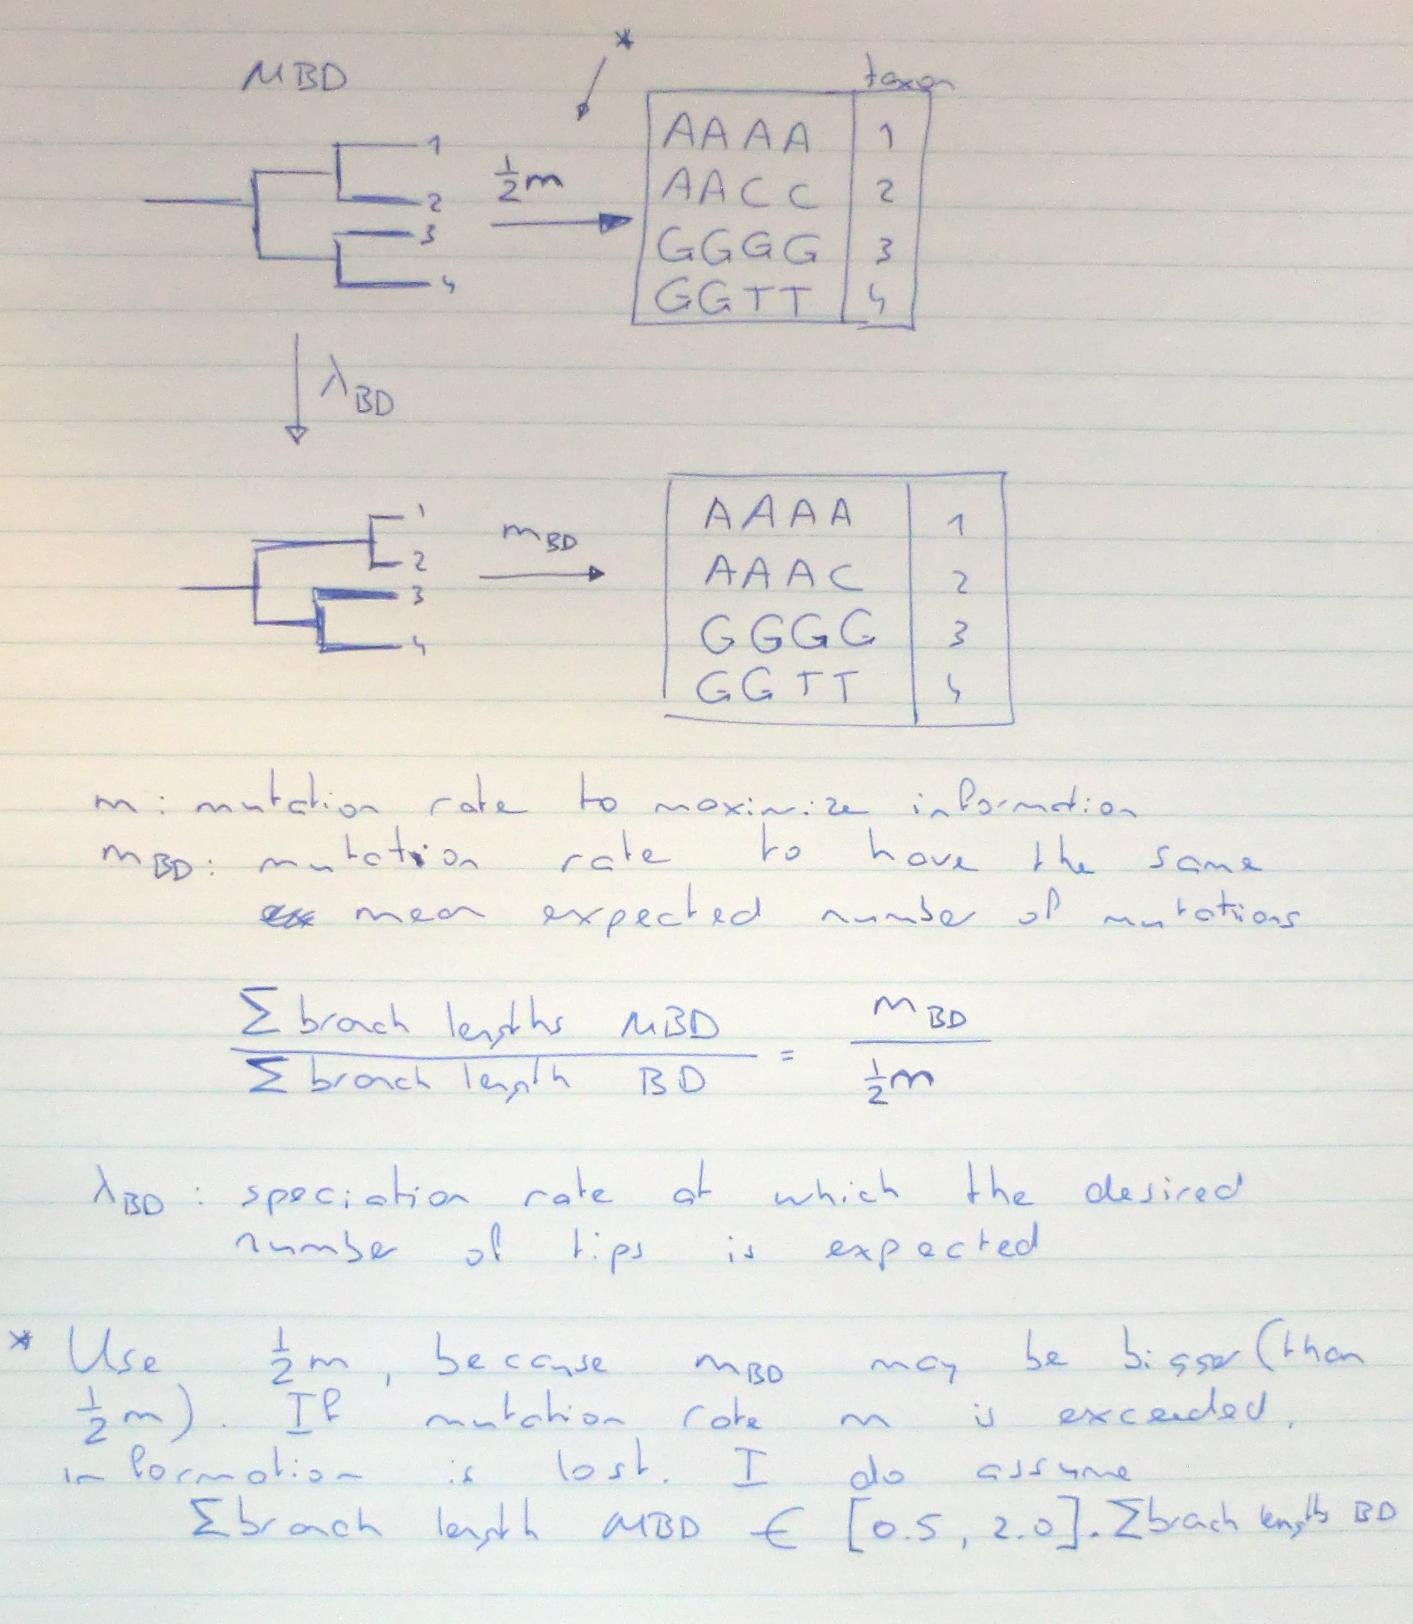
\includegraphics[width=\textwidth]{mbd.jpg}
  \caption{
    How to create twin trees and alignments. 
    From a focal MBD tree, a twin tree is produced as 
    such: (1) estimate the $\lambda_{BD}$ to get 
    the same expected number of tips, (2) simulate a BD tree 
    with that amount of tips (discard trees with different number of tips), 
    (3) estimate a mutation rate to get an alignment 
    with the same expected number of mutations, (4) simulate alignments 
    with that amount of mutations (discard those that don't, 
    the picture shows an alignment that should be discarded) 
  }
\end{figure}

\item We explained how we set the parameters for each twin BD tree. 
Using this rules we generate a BD dataset. 
We repeat the analysis, producing alignments for each tree 
and subsequently using BEAST to produce a posterior for each of them.

\subsection{Measuring the inference error}

\item So far we have simulated two datasets of trees under the two models: 
$\{T_{i}^{BD}\}_{i=1}^{N_{S}}$ and $\{T_{i}^{MBD}\}_{i=1}^{N_{S}}$.
We used them to generate a dataset of alignments for each model: $\{X^{BD}_{i}\}_{i=1}^{N_{S}}$ and $\{X^{MBD}_{i}\}_{i=1}^{N_{S}}$. From each dataset we produced a posterior distribution from a BD prior: 
$P_{i}(\theta | X^{BD}_{i}, BD)$ and $P_{i}(\theta | X^{MBD}_{i}, BD)$.
\gio{
  1) We might want to rename the models, e.g. BD = (0) and MBD = (1). 
  These names with capital letters are too big and ugly;
}
\richel{
  I would strongly prefer MBD and BD, as I feel replacing the big ugly 
  capital letters by short pretty numbers hurts readability even more 
}

\item To compare the results for the two models we measure the inference 
error using the nLTT statistic between known/true tree and 
posterior/inferred trees (\cite{nltt}). 
To obtain such statistics the procedure is the following:

- From each tree $T_{i,j}^{M}$ (with $j=1,...,N_{S}$) 
  belonging to the posterior $P_{i}(\theta | X^{M}_{i}, BD)$ 
  and relative to the model $M$, we extrapolate the lineage-through-time (LTT), 
  in other words we measure the number of species as a function of 
  time $n_{i,j}(t)$. To allow a comparison we normalize dividing by the 
  maximum number of species of each tree, i.e. the number of tips at the 
  present $N_{i,j}(t)=\frac{n_{i,j}(t)}{n^{max}_{i,j}}$. We then define the 
  nLTT measure as

$nLTT_{i,j} = \int_{0}^{T} | N_{i,j}(t) - N_{T_{i}} | dt$

\gio{I am running out of letters :(}
\richel{Haha! I suggest to use the same equation and symbols 
  as equation 1 in
  the nLTT article of Janzen, Hoehna and Etienne, 2015:
}

$$
\Delta nLTT = \int_{0}^{1} | nLTT_1(t) - nLTT_2{t} | dt
$$

\subsection{Model selection}

\end{itemize}
%%%%%%%%%%%%%%%%%%%%%%%%%%%%%%%%%%%%%%%%%%%%%%%%%%%%%%%%%%%%%%%%%%%%%%%%%%%%%%%%

%%%%%%%%%%%%%%%%%%%%%%%%%%%%%%%%%%%%%%%%%%%%%%%%%%%%%%%%%%%%%%%%%%%%%%%%%%%%%%%%
\section{Results}
\begin{itemize}

\item

\item

\end{itemize}
%%%%%%%%%%%%%%%%%%%%%%%%%%%%%%%%%%%%%%%%%%%%%%%%%%%%%%%%%%%%%%%%%%%%%%%%%%%%%%%%

%%%%%%%%%%%%%%%%%%%%%%%%%%%%%%%%%%%%%%%%%%%%%%%%%%%%%%%%%%%%%%%%%%%%%%%%%%%%%%%%
% Bibliography % MEE style
\bibliographystyle{mee}
\bibliography{article}
%%%%%%%%%%%%%%%%%%%%%%%%%%%%%%%%%%%%%%%%%%%%%%%%%%%%%%%%%%%%%%%%%%%%%%%%%%%%%%%%

%%%%%%%%%%%%%%%%%%%%%%%%%%%%%%%%%%%%%%%%%%%%%%%%%%%%%%%%%%%%%%%%%%%%%%%%%%%%%%%%
\appendix


%%%%%%%%%%%%%%%%%%%%%%%%%%%%%%%%%%%%%%%%%%%%%%%%%%%%%%%%%%%%%%%%%%%%%%%%%%%%%%%%


\end{document}